\documentclass[12pt,A4paper]{article}
%\pdfoutput=1

\usepackage{multirow}
\usepackage{cite}
\usepackage{hyperref}
\usepackage{slashed}
\usepackage{graphicx}
    \usepackage{amsmath}
    \usepackage{caption}
    \usepackage{subcaption}
    \usepackage{cancel}
    \usepackage{etoolbox} % provides \patchcmd macro
    \makeatletter % modify the "headings" page style
    \patchcmd{\ps@headings}{{\slshape
ightmark}\hfil	hepage}{	hepage\hfil}{}{}
    \makeatother
    \pagestyle{headings}
\usepackage{listings}
\usepackage{color}
\usepackage{appendix}

\textwidth 170mm
\textheight 220mm
\oddsidemargin -5mm
\evensidemargin 5mm
\topmargin -16pt

\newcommand{\colspacea}{\hphantom{33333333}}
\newcommand{\colspaceb}{\hphantom{33333333}}
\newcommand{\colspacec}{\hphantom{33333333}}
\newcommand{\colspace}{\hphantom{33333333333}}


\newcommand{\xspace}{~}
\newcommand{\GeV}{\ensuremath{\,\text{Ge\hspace{-.08em}V}}\xspace}
\newcommand{\PSGczDo}{\ensuremath{\widetilde{\chi}^{0}_{1}}\xspace} % neutralino
\newcommand{\Pp}{\ensuremath{p}}
\newcommand{\PSg}{\ensuremath{\widetilde{g}}}
\newcommand{\PQq}{\ensuremath{q}}
\newcommand{\cPqt}{\ensuremath{t}}
\newcommand{\cPq}{\ensuremath{q}}
\newcommand{\cPqb}{\ensuremath{b}}
\newcommand{\PAQq}{\overline{\ensuremath{q}}}
\newcommand{\cPaqt}{\overline{\ensuremath{t}}}
\newcommand{\cPaqb}{\overline{\ensuremath{b}}}
\newcommand{\PSQ}{\ensuremath{\widetilde{q}}}
\newcommand{\PSGcz}{\ensuremath{\widetilde{\chi_0^1}}}
\newcommand{\qqbar}{\ensuremath{\PQq\PAQq}\xspace}
%\newcommand{\mgluino}{\ensuremath{m_{\PSg}}\xspace}
\newcommand{\HT}{\ensuremath{H_{\mathrm T}}\xspace}
\newcommand{\MHT}{\ensuremath{H_{\mathrm T}^{\text{miss}}}\xspace}
\newcommand{\njets}{\ensuremath{N_{\text{jet}}}~}
\newcommand{\nbjets}{\ensuremath{N_{\text{b-jet}}}~}
\newcommand{\mgluino}{\ensuremath{m_{\PSg}}\xspace}
\newcommand{\msquark}{\ensuremath{m_{\PSQ}}\xspace}
%\newcommand{\mlsp}{\ensuremath{m_{{\PSGcz}_1}}\xspace}
\newcommand{\tbbar}{\ensuremath{\cPqt\cPaqb}\xspace} % t-bbar
\newcommand{\ttbar}{\ensuremath{t\overline{t}}\xspace} % t-tbar
\newcommand{\bbbar}{\ensuremath{b\overline{b}}\xspace} % b-bbar
\newcommand{\sTop}{\ensuremath{\widetilde{t}}\xspace}
\newcommand{\sBot}{\ensuremath{\widetilde{b}}\xspace}
\newcommand{\sQua}{\ensuremath{\widetilde{q}}\xspace}
\newcommand{\PASQt}{\ensuremath{\overline{\widetilde{t}}}\xspace} % anti stop
\newcommand{\PASQb}{\ensuremath{\overline{\widetilde{b}}}\xspace} % anti sbottom
\newcommand{\PASQ}{\ensuremath{\overline{\widetilde{q}}}\xspace} % anti squark


\newcommand{\neles}{\ensuremath{N_{\text{electron}}}\xspace}
\newcommand{\nmuons}{\ensuremath{N_{\text{muon}}}\xspace}
\newcommand{\nisomuons}{\ensuremath{N_{\text{isolated tracks}}^{\text{(muon)}}}\xspace}
\newcommand{\nisoeles}{\ensuremath{N_{\text{isolated tracks}}^{\text{(electron)}}}\xspace}
\newcommand{\nisohads}{\ensuremath{N_{\text{isolated tracks}}^{\text{(hadron)}}}\xspace}
\newcommand{\dpmht}[1]{\ensuremath{\Delta\phi_{\MHT,j_{#1}}}\xspace}


\newcommand{\mulobs}{$\sigma^{\mathrm{UL}}_{\mathrm{obs}}$}
\newcommand{\ulobs}{\sigma^{\mathrm{UL}}_{\mathrm{obs}}}
\newcommand{\mulexp}{$\sigma^{\mathrm{UL}}_{\mathrm{exp}}$}
\newcommand{\ulexp}{\sigma^{\mathrm{UL}}_{\mathrm{exp}}}
\newcommand{\mtheo}{$\sigma^{\mathrm{pred}}_{\mathrm{theo}}$}
\newcommand{\theo}{\sigma_{\mathrm{pred}}^{\mathrm{theo}}}

\newcommand{\lumi}{\mathcal{L}}
\newcommand{\twomm}{\hspace{2mm}}
\newcommand{\neu}{{\widetilde{\chi}_1^0}}

\newcommand{\go}{{\widetilde{g}}}
\newcommand{\sq}{{\widetilde{q}}}
\newcommand{\mmsq}{$m_{\widetilde{q}}$}
\newcommand{\msq}{m_{\widetilde{q}}}
\newcommand{\mlsp}{m_{\widetilde{\chi}}}
\newcommand{\mmlsp}{$m_{\widetilde{\chi}}$}
\newcommand{\mgo}{m_{\widetilde{g}}}
\newcommand{\mmgo}{$m_{\widetilde{g}}$}

\definecolor{dkgreen}{rgb}{0,0.6,0}
\definecolor{gray}{rgb}{0.5,0.5,0.5}
\definecolor{mauve}{rgb}{0.58,0,0.82}
\lstset{ %
  language=C++,                % the language of the code
  basicstyle=\footnotesize,           % the size of the fonts that are used for the code
  %  numbers=left,                   % where to put the line-numbers
  %  numberstyle=\tiny\color{gray},  % the style that is used for the line-numbers
  %  stepnumber=2,                   % the step between two line-numbers. If it's 1, each line
  % will be numbered
  %  numbersep=5pt,                  % how far the line-numbers are from the code
  backgroundcolor=\color{white},      % choose the background color. You must add \usepackage{color}
  showspaces=false,               % show spaces adding particular underscores
  showstringspaces=false,         % underline spaces within strings
  showtabs=false,                 % show tabs within strings adding particular underscores
  frame=single,                   % adds a frame around the code
  rulecolor=\color{black},        % if not set, the frame-color may be changed on line-breaks within not-black text (e.g. commens (green here))
  tabsize=2,                      % sets default tabsize to 2 spaces
  captionpos=b,                   % sets the caption-position to bottom
  breaklines=true,                % sets automatic line breaking
  breakatwhitespace=false,        % sets if automatic breaks should only happen at whitespace
  title=\lstname,                   % show the filename of files included with \lstinputlisting;
  % also try caption instead of title
  keywordstyle=\color{blue},          % keyword style
  commentstyle=\color{dkgreen},       % comment style
  stringstyle=\color{mauve},         % string literal style
  escapeinside={\%*}{*)},            % if you want to add a comment within your code
  morekeywords={*,\dots}               % if you want to add more keywords to the set
}


\title{Validation of the \texttt{MadAnalysis 5} implementation of CMS-EXO-16-012}
\author{Jiwon Park\footnote{jiwon.park@cern.ch} , Seohyun Ahn\footnote{klar.wind0425@gmail.com} (Hanyang University) \and Wenxing Zhang\footnote{zhangwenxing@itp.ac.cn} (ITP of Chinese Academy of Science)\\ 
\date{\today}
}

\begin{document}
        \maketitle

%\clearpage
%%%%%%%%%%%%%%%%%%%%%%%%%%%%%%%%%%%%%%%%%%%%%%%%%
\section{Introduction}
\indent In this document, the \texttt{MadAnalysis 5 v1.6} \cite{ref:ma51,ref:ma52,ref:ma53} implementation of search for associated production of dark matter with a
Higgs boson decaying to \bbbar or $\gamma\gamma$ at $\sqrt{s} = 13$ TeV (2.3 fb$^{-1}$)\cite{ref:paper} is validated.

 This paper is written in the context of $Z'$-two-Higgs-doublet model, where a high-mass resonance $Z'$ decays into a pseudoscalar boson $A$ and a CP-even scalar Higgs boson, and the A decays to a pair of dark matter particles, as shown in \ref{fig:model1}. For further theoretical aspects of this model, see the paper \cite{ref:theory}

\begin{figure}[h!]
    \centering
    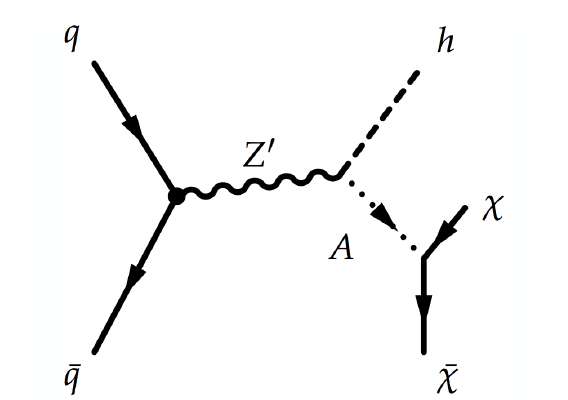
\includegraphics[width=0.5\textwidth]{img/model_fig1.png}
    \caption{The $Z'$ 2HDM model with pseudoscalar $A$}
    \label{fig:model1}
\end{figure}

%%%%%%%%%%%%%%%%%%%%%%%%%%%%%%%%%%%%%%%%%%%%%%%%%
%%%%%%%%%%%%%%%%%%%%%%%%%%%%%%%%%%%%%%%%%%%%%%%%%
\section{Description of the implementation}
\subsection{Objects definition}
There are several selections for photon identification. Cut based photon identification with loose working point is applied. The selections are presented in the photon id paper from CMS, as well as PAS EXO-16-012\cite{ref:photonid, ref:paper}. Isolation is computed in a area with angular separation $\Delta R = 0.3$ ($\Delta R = \sqrt{(\Delta\eta)^2+(\Delta\phi)^2}$). 

First, the events with diphoton mass cut where $m_{\gamma\gamma} > 95$ GeV and asymmetric $p_T$ threshold (30 and 18 GeV) are selected. 
Next, to reject fake photons, cuts on energy deposit in Hadronic Calorimeter(HCAL) over energy deposit in Electromagnetic Calorimeter(ECAL), which denoted as H/E, is required to be less than 0.1. Isolation cuts for charged hadron (Iso$_{ch}$), neutral hadron (Iso$_{Neu}$), and photon (Iso$_{\gamma}$) is also applied. For neutral particles, isolations are computed with $\rho$ correction to take into account the dependence of the pileup transverse energy density on pseudorapidity, where $\rho$ is the median of the transverse energy density per unit area.

\begin{center}
\begin{table}[h!]
	\begin{tabular}{c c c}
	\hline
	Variable & Barrel Selection & Endcap Selection\\
	\hline
	H/E& \multicolumn{2}{c}{ $< $0.1}\\
	Iso$_{ch}$ [GeV]& $<$ 3.32& $<$ 1.97\\
	$\rho$ corrected Iso$_{Neu}$ [ GeV ]& $< 1.92 + 0.14 p_T + 0.000019(p_T)^2$& $< 11.86 + 0.0139 p_T + 0.000025(p_T)^2$\\

	$\rho$ corrected Iso$_{\gamma}$ [ GeV ]& $< 0.81 + 0.0053 p_T$& $< 0.83 + 0.0034 p_T$\\
	\hline
	\end{tabular}
	\caption{Value of each variable used in barrel and endcap photon identification} \vspace*{-20pt}
\end{table}
\end{center}

\subsection{Signal selections}
After these selections, we applied additional cuts to maximize the expected significance for each $Z'$ mass point. The chosen kinematic selections include $p_{T_1}/m_{\gamma\gamma} > 0.5$ and $p_{T_2}/m_{\gamma\gamma} > 0.25$, for leading photon $\gamma_1$ and subleading photon $\gamma_2$. Moreover we imposed a diphoton transverse momentum and missing transverse momentum cut, $p_{T_{\gamma\gamma}} > 90$ GeV and $p_T^{miss} > 105$ MeV.

In addition, two more cuts are applied to enhance the signal over background discrimination and to veto events with mismeasured $p_T^{miss}$ (transverse momentum component of $E^{miss}_T$).
\begin{itemize}
	\item $|\Delta\phi(\gamma\gamma,\,p_T^{miss})| > 2.1$
	\item $min(|\Delta\phi(jet,\,\vec p_T^{miss})|) > 0.5$ for all jets in the event with $p_T > 50$ GeV where jets are reconstructed with the clustering of PF candidates by means of the anti-kt algorithm with a distance parameter of 0.4.
\end{itemize}

Finally we defined a signal region (SR), where $120 < m_{\gamma\gamma} < 130$ GeV and $p_T^{miss} > 105$ MeV.


%%%%%%%%%%%%%%%%%%%%%%%%%%%%%%%%%%%%%%%%
\section{Validation}
\subsection{Event Generation}
To generate a signal sample, \href{http://rkhurana.web.cern.ch/rkhurana/monoH/models/}{model UFO file} is provided by CMS. From the \href{https://github.com/cms-sw/genproductions/tree/master/bin/MadGraph5_aMCatNLO/cards/production/13TeV/monoHiggs/Zp2HDM/Zprime_A0h_A0chichi}{CMS genproduction github repository}\cite{ref:gitgen} one can retrieve the cards used for \texttt{MadGraph MG5\_aMC}\cite{ref:mg5} event generation for each mass point of $Z'$. 
The \href{https://github.com/cms-sw/genproductions/blob/mg240/bin/MadGraph5_aMCatNLO/cards/production/13TeV/monoHiggs/Zp2HDM/Zprime_A0h_A0chichi/Zprime_A0h_A0chichi_MZp600_MA0300/Zprime_A0h_A0chichi_MZp600_MA0300_run_card.dat}{run card} used in \texttt{MadGraph MG5\_aMC} and \href{https://github.com/cms-sw/genproductions/blob/mg240/bin/MadGraph5_aMCatNLO/cards/production/13TeV/monoHiggs/Zp2HDM/Zprime_A0h_A0chichi/Zprime_A0h_A0chichi_MZp600_MA0300/Zprime_A0h_A0chichi_MZp600_MA0300_proc_card.dat}{process card} were retrieved from the repository. 
In \texttt{MadGraph MG5\_aMC} $Z'$ particle is produced via the proton-proton collision and forced to decay into a standard model Higgs boson and a pseudoscalar boson $A$. 
Next, $A$ is made to decay into two dark matter particles. The decay of Higgs boson into $\gamma\gamma$ is handled in \texttt{Pythia 8}\cite{ref:pythia}. This paper is focused on the H$\rightarrow\gamma\gamma$ only.

Also some \href{https://github.com/cms-sw/genproductions/blob/mg240/bin/MadGraph5_aMCatNLO/cards/production/13TeV/monoHiggs/Zp2HDM/Zprime_A0h_A0chichi/Zprime_A0h_A0chichi_MZp600_MA0300/Zprime_A0h_A0chichi_MZp600_MA0300_customizecards.dat}{custom settings} were applied according to the mass range of $Z'$ ($M_{Zp} = 600 \sim 2500$). 
Mass of $A$ is fixed to $300$ GeV. The coupling to dark matter was chosen to be 1\cite{ref:dm}. 
Higgs boson mass is set to $M_H = 125$ GeV in \texttt{Pythia 8} and only the H$\rightarrow\gamma\gamma$ decay is turned on.
The default pythia tunes which commonly used in CMS to match Monte Carlo samples to the data are also applied. These run, process, and pythia cards can be found in CMS software github repository\cite{ref:gitgen}.
\begin{itemize}
    \item \href{https://github.com/cms-sw/cmssw/blob/CMSSW_7_1_9_patch/Configuration/Generator/python/Pythia8CUEP8M1Settings_cfi.py}{Pythia8CUEP8M1Settings},
    \item \href{https://github.com/cms-sw/cmssw/blob/CMSSW_7_2_X/Configuration/Generator/python/Pythia8CommonSettings_cfi.py}{Pythia8CommonSettings}.
%    \item \href{https://github.com/cms-sw/genproductions/blob/master/python/ThirteenTeV/monoHiggs/pythia8_hadronizer_nomatching_Haa_cff.py}{The genfragment file is used.}
\end{itemize}


For detector simulation, we used \texttt{Delphes 3}\cite{ref:delphes} with latest version of delphes card used for EXO-16-037 recasting\cite{ref:exo037}. Compared with default setting, b tagging efficiency and areas for computing lepton and photon isolation are changed\cite{ref:beff,ref:photonid}. We introduced b tagging efficiency formula used for cMVAv2 loose working point where b tagging efficiency is about 83\% and misidentification probability is about 10\%. Also we added some lines to make neutralino not to deposit energy on calorimeter. 

%%%%%%%%%%%%%%%%%%%%%%%%%%%%%%%%%%%%%%%%%%%%%%%%%
\subsection{Comparision with official results}
 CMS did not provide a detailed cutflow. Here we present the product of acceptance and efficiency for signal in the SR for each mass point only. The error is defined as 
\begin{align*}
	(1-(A\cdot\epsilon)^{MA5}/(A\cdot\epsilon)^{CMS} \,(\%).
\end{align*}

\vskip 10pt


\begin{center}
\begin{tabular}{c c c c}
\hline
\multicolumn{4}{c}{Acceptance $\times$ efficiency $(A \cdot \epsilon)$}\\
\hline
$m_{Z_p}$ (GeV)& CMS EXO-16-012& MA5& Error\\
\hline
600& 0.317 $\pm$ 0.004& 0.355 $\pm$ 0.001& -11 \%\\%35512
800& 0.399 $\pm$ 0.004& 0.451 $\pm$ 0.001& -13 \%\\%45140
1000& 0.444 $\pm$ 0.004& 0.494 $\pm$ 0.001& -8.2 \%\\%49355
1200& 0.474 $\pm$ 0.004& 0.513 $\pm$ 0.001& -0.6 \%\\%51302
1400& 0.492 $\pm$ 0.004& 0.515  $\pm$ 0.001& -4.7 \%\\%51545
1700& 0.493 $\pm$ 0.004& 0.494 $\pm$ 0.001& -0.2 \%\\%49442
2000& 0.351 $\pm$ 0.004& 0.355 $\pm$ 0.001& -1.1 \%\\%35451
2500& 0.213 $\pm$ 0.004& 0.208 $\pm$ 0.001& 2.3 \%\\%20759
\hline
\vspace*{20pt}
\end{tabular}
\end{center}

Since missing transverse energy is important, we plotted only $ p_T^{miss}$ and $m_{\gamma\gamma}$. For this step, we made plot without normalization. For both plots from paper, the product of signal cross section and branching fraction is set to 1 fb. But exact branching ratios are not provided, so we compared shapes only.

\begin{figure}[h!]
\centering
\begin{minipage}{.5\textwidth}
  \centering
  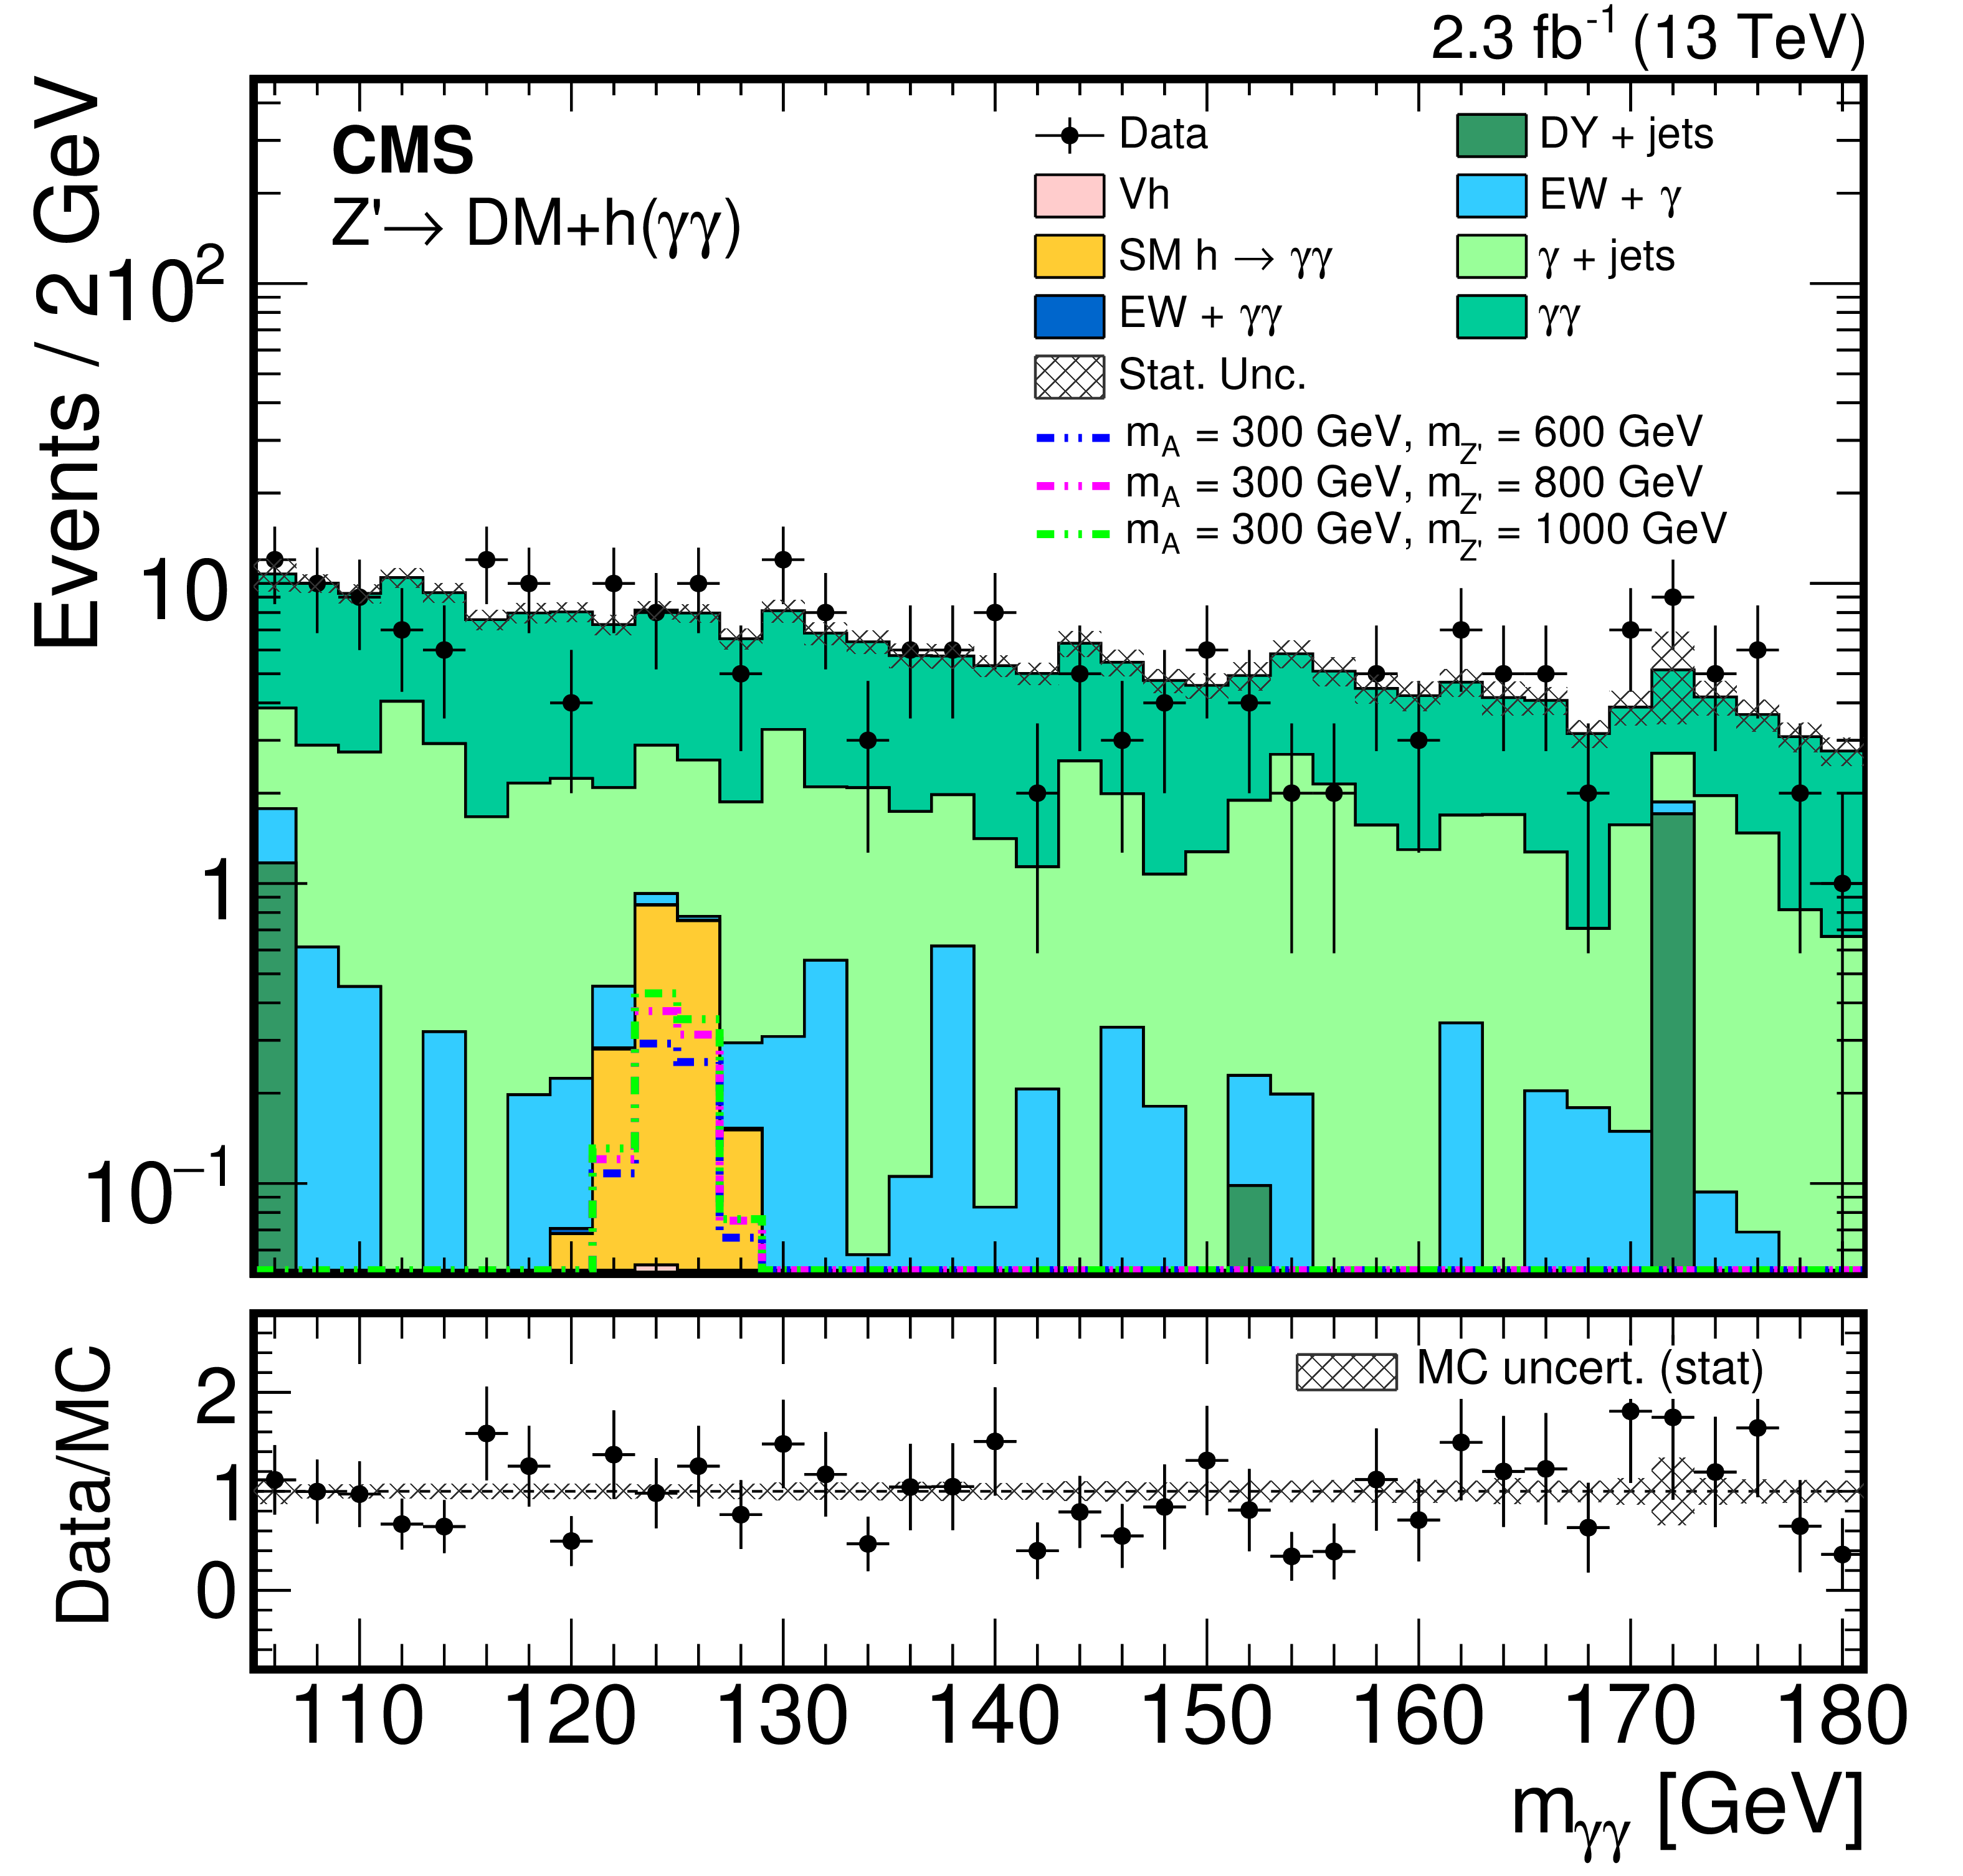
\includegraphics[scale=0.08]{img/CMS-EXO-16-012_Figure_007-a.png}
\end{minipage}%
\begin{minipage}{.5\textwidth}
  \centering
   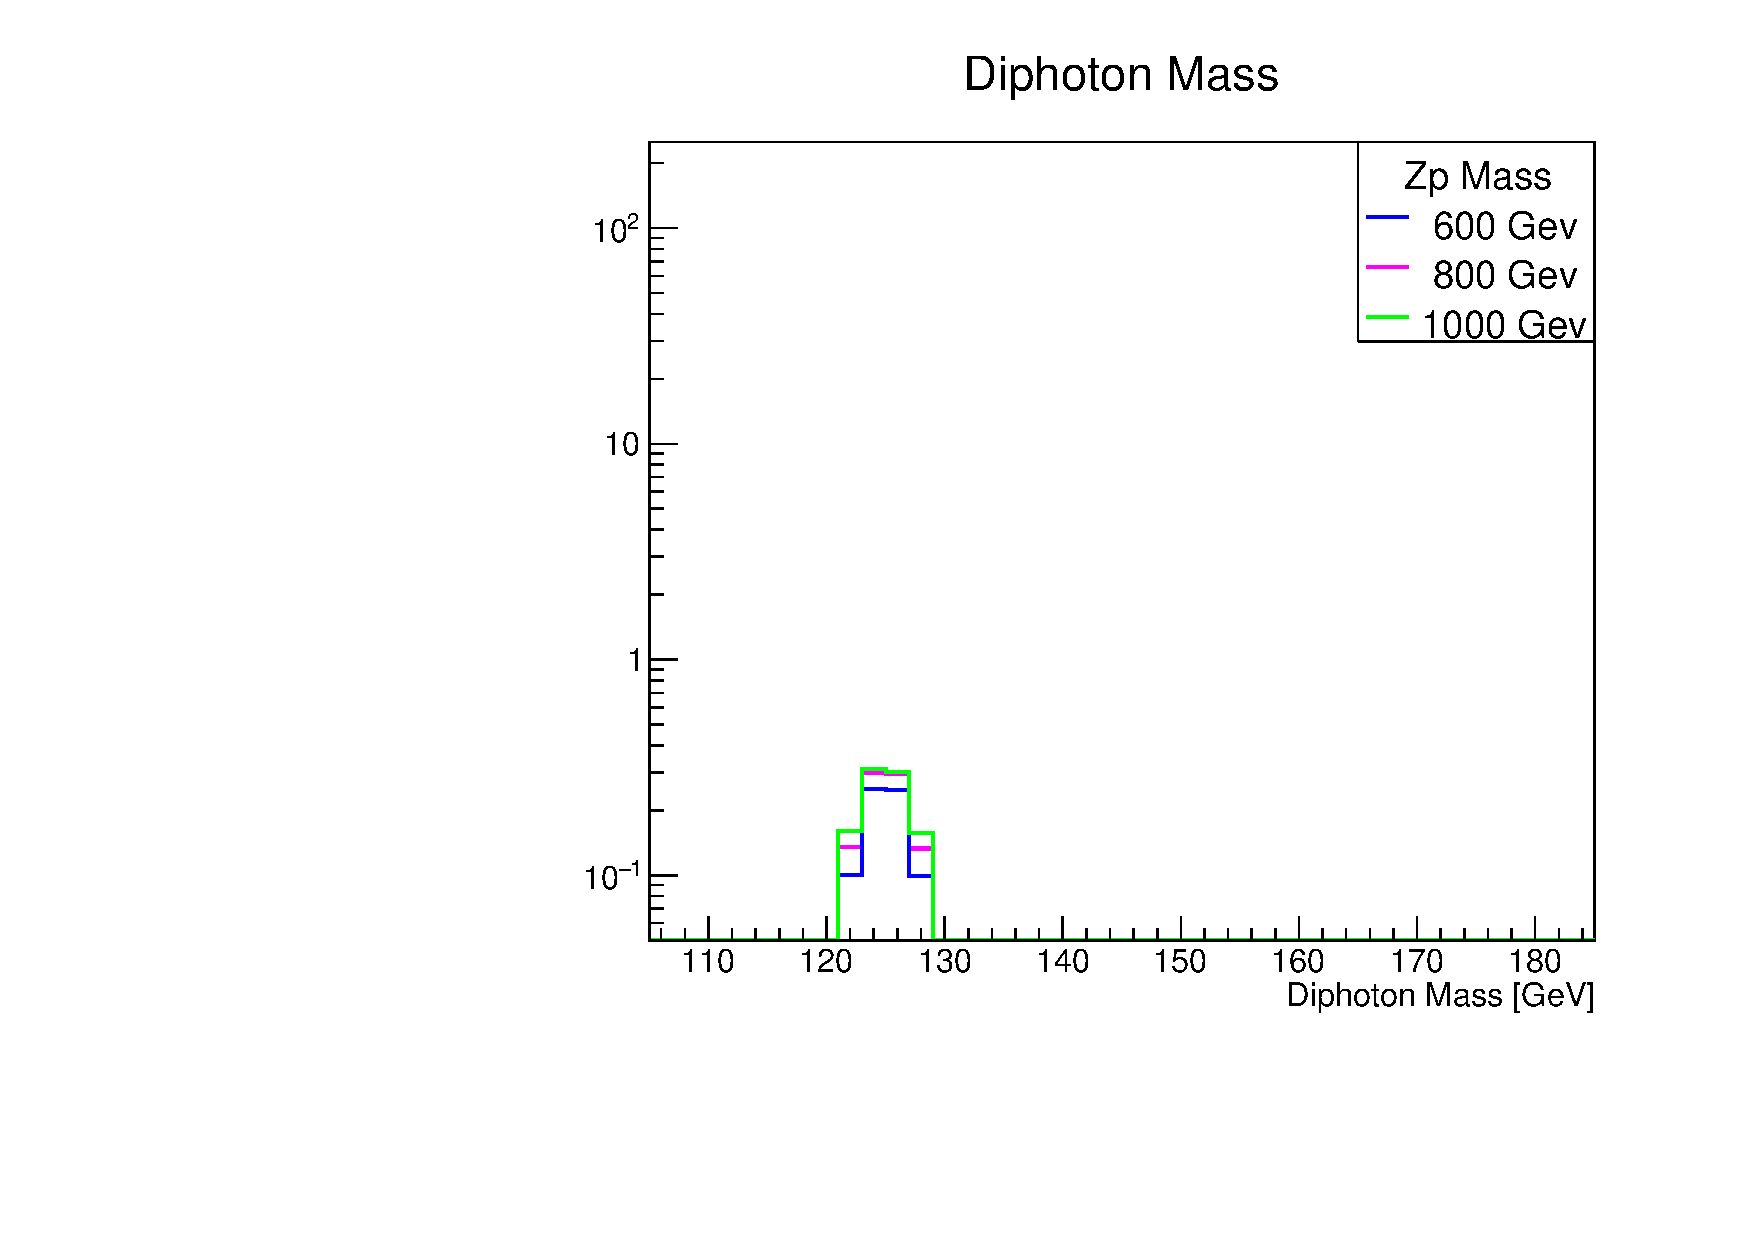
\includegraphics[scale=0.45]{img/MZp_M.pdf}
\end{minipage}
\caption{Distribution of $m_{\gamma\gamma}$ (left)\cite{ref:paper} in events passing all selection criteria except the $m_{\gamma\gamma}$ and $p_T^{miss}$ requirement. For the left plot, the product of signal cross section and branching fraction is set to 1 fb.}
\end{figure}

\begin{figure}[h!]
\centering
	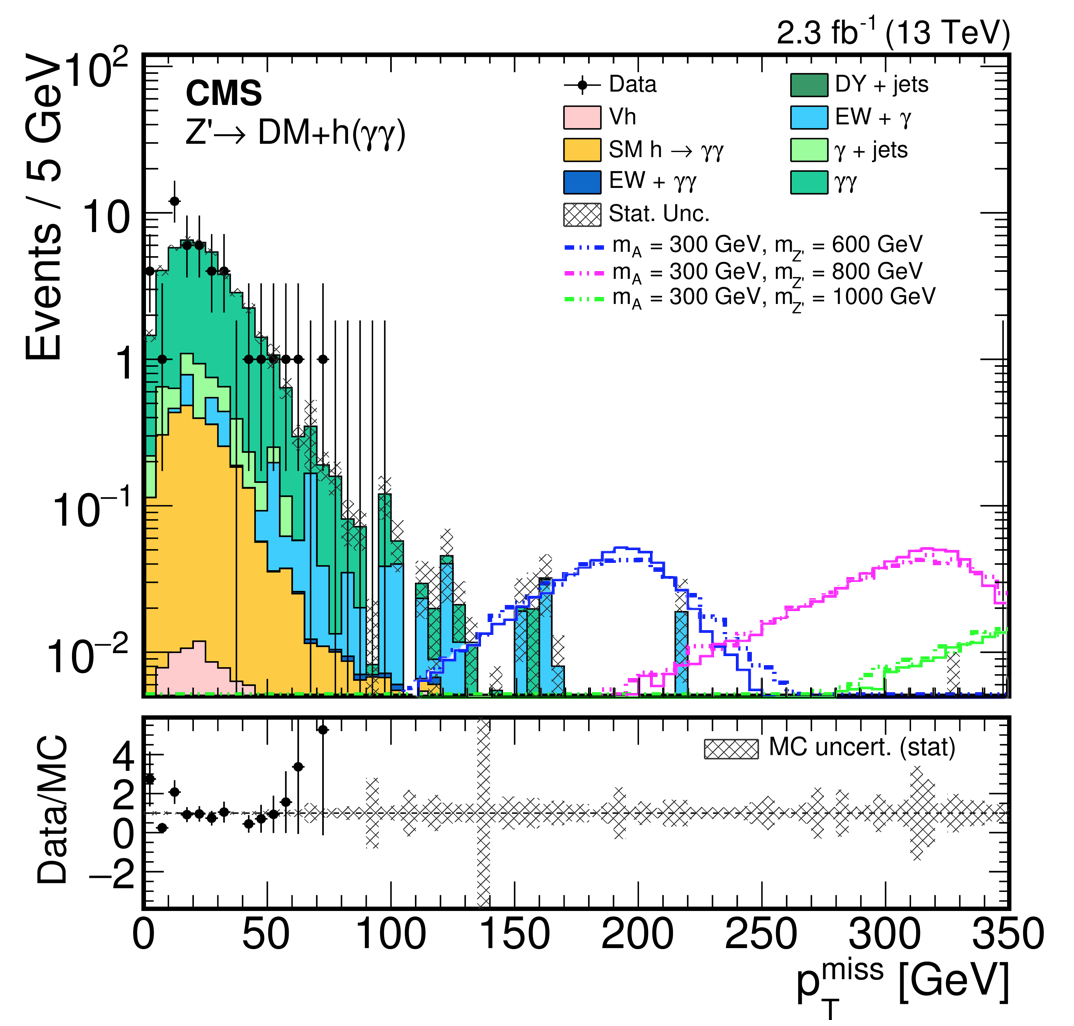
\includegraphics[scale=0.6]{img/overlayed.png}
\caption{Distribution of $p_T^{miss}$ for events passing all selection criteria including $120 \textrm{GeV} < m_{\gamma\gamma} < 130 \textrm{GeV}$ except $p_T^{miss}$ requirement. Dotted lines are CMS official results\cite{ref:paper} and solid lines are recast results. Since normalization factors are not provided, recast results are plotted for shape comparison purpose only.}
\end{figure}

\clearpage

\begin{thebibliography}{5}\vspace{-7pt}

\bibitem{ref:ma51} E. Conte, B. Fuks, and G. Serret, ``MadAnalysis 5, a user-friendly framework for collider phenomenology'' Comput.Phys.Commun. 184, 222 (2013), \href{https://arxiv.org/abs/1206.1599}{arxiv:1206.1599}.

\bibitem{ref:ma52} E. Conte, B. Dumont, and B. Fuks, C. Wymant, ``Designing and recasting LHC analyses with MadAnalysis 5''
Eur. Phys .J. C 74, 3103 (2014), \href{https://arxiv.org/abs/1405.3982}{arxiv:1405.3982}

\bibitem{ref:ma53} B. Dumont et al, ``Towards a public analysis database for LHC new physics searches using MadAnalysis 5'', Eur. Phys .J. C 75, 56 (2014), \href{https://arxiv.org/abs/1407.3278}{arxiv:1407.3278}

\bibitem{ref:paper} CMS Collboration, ``Search for associated production of dark matter with a Higgs boson decaying to b-bbar or gamma-gamma at sqrt(s) = 13 TeV'' 2017, \href{https://arxiv.org/abs/1703.05236}{arXiv:1703.05236} \href{http://cms-results.web.cern.ch/cms-results/public-results/publications/EXO-16-012/}{CMS-PAS-EXO-16-012}

\bibitem{ref:theory} A. Berlin, et al. ``Mono-Higgs Detection of Dark Matter at the LHC'', JHEP 06 (2014) 078, \href{https://arxiv.org/abs/1402.7074}{arXiv:1402.7074}

\bibitem{ref:mg5} J. Alwall et al., ``The automated computation of tree-level and next-to-leading order differential cross sections, and their matching to parton shower simulations'', JHEP 07 (2014) 079, \href{https://arxiv.org/abs/1405.0301}{arXiv:1405.0301}.

\bibitem{ref:pythia} T. Sjstrand et al., ``An Introduction to PYTHIA 8.2'', Comput. Phys. Commun. 191, 159 (2015) \href{https://arxiv.org/abs/1410.3012}{arXiv:1410.3012}.

\bibitem{ref:dm} D. Abercrombie, ``Dark Matter Benchmark Models for Early LHC Run-2 Searches: Report of the ATLAS/CMS Dark Matter Forum'', \href{https://arxiv.org/abs/1507.00966}{arXiv:1507.00966}.

\bibitem{ref:gitgen} \url{https://github.com/cms-sw/genproductions}

\bibitem{ref:delphes} J. Favereau, et al. ``DELPHES 3, A modular framework for fast simulation of a generic collider experiment'', JHEP 02 (2014) 057, \href{https://arxiv.org/abs/1307.6346}{arXiv:1307.6346}.

\bibitem{ref:beff} CMS Collboration, ``
Identification of b quark jets at the CMS Experiment in the LHC Run 2'', CMS PAS BTV-15-001.


\bibitem{ref:exo037} B. Fuks, M. Zumbihl, CMS-EXO-16-037 recasting \url{https://madanalysis.irmp.ucl.ac.be/wiki/PublicAnalysisDatabase}

\bibitem{ref:photonid} CMS Collaboration, ``Performance of Photon Reconstruction and Identification with the CMS Detector in Proton-Proton Collisions at sqrt(s) = 8 TeV'', JINST 10 (2015), \href{https://arxiv.org/abs/1502.02702}{arXiv:1502.02702}

\end{thebibliography}


\end{document}
